\documentclass{article}

% if you need to pass options to natbib, use, e.g.:
%     \PassOptionsToPackage{numbers, compress}{natbib}
% before loading neurips_2019

% ready for submission
% \usepackage{neurips_2019}

% to compile a preprint version, e.g., for submission to arXiv, add add the
% [preprint] option:
%     \usepackage[preprint]{neurips_2019}

% to compile a camera-ready version, add the [final] option, e.g.:
  %  \PassOptionsToPackage{numbers}{natbib}
      \usepackage[pdftex]{graphicx} 
     \usepackage[final]{neurips_2019}

% to avoid loading the natbib package, add option nonatbib:
%    \usepackage[nonatbib]{neurips_2019}

\usepackage[utf8]{inputenc} % allow utf-8 input
\usepackage[T1]{fontenc}    % use 8-bit T1 fonts
\usepackage{hyperref}       % hyperlinks
\usepackage{url}            % simple URL typesetting
\usepackage{booktabs}       % professional-quality tables
\usepackage{amsfonts}       % blackboard math symbols
\usepackage{nicefrac}       % compact symbols for 1/2, etc.
\usepackage{microtype}      % microtypography

\title{Agency vs Communion in letters, memoirs, and autobiographies  2019}

% The \author macro works with any number of authors. There are two commands
% used to separate the names and addresses of multiple authors: \And and \AND.
%
% Using \And between authors leaves it to LaTeX to determine where to break the
% lines. Using \AND forces a line break at that point. So, if LaTeX puts 3 of 4
% authors names on the first line, and the last on the second line, try using
% \AND instead of \And before the third author name.

\author{%
  Michael Hearn, Aditya Patel, and  Ahn Tran\\ %\thanks{Use footnote for providing further information
   % about author (webpage, alternative address)---\emph{not} for acknowledging
%    funding agencies.} \\
  Department of Computer Science\\
  University of Georgia\\
  Athens, GA 30602 \\
  \texttt{michaeljosephhearn@gmail.com}, {adipat@uga.edu} , {adt86418@uga.edu}\\
}
\begin{document}

\maketitle

\begin{abstract}
   We explored methodologies for generating and visualizing metrics of agency and communion in various documents.
   Using synonyms of labels thematically connected to agency and communion and cross referencing them with vectorized word similarity we were able to create a methodology for scoring words based on their similarity to the theme of agency and communion. Using the scored words we are able to mark words of interest in the text most likely to be associated with the agency and communion themes throughout the document.
    
\end{abstract}

\section{Introduction}

Agency and Communion are the two basic styles for describing how individuals relate to their social milieu. David Bakan, an American psychologist, identifies agency and communion as two elementary modal qualities of living forms. He writes “Agency manifests itself in the formation of separations, isolation, alienation, aloneness, the urge to master, and the repression of thought, feeling, and impulsive; communion is manifested in a sense of being at one with other organisms, a lack of separations, the lack and removal of repression, contact, openness, and union, and noncontractual cooperation.” [1](Bakan, 1966, page. 15). Thus, agency and communion both complement each other. People high in agency are focused on their individual accomplishments, whereas people high in communion are more focused on societal or a group’s accomplishments and welfare.

For healthy personality development, conventional perspective emphasizes on agency, individuation and independence. Though some theorists does not agree to this and believes that both individuation and tendency to relate to others, advances personality development even more. While some theorists believe that as we age and become more mature our own agency and communion sides balances out and eventually we become more communal.

Our aim in this project was to find the amount of agency and communion in certain autobiographies, memoirs and letters mainly from 19th and 20th century fetched from Project Gutenberg (gutenberg.org). Our group members from English department gave us an article [2] that gave us a list of words whose presence represents agency and communion. We used these words for further computation of the data that they gave us. Processing the memoirs, letters and autobiographies gives us an idea of how much change comes in the patterns between agency and communion over the author's life or during certain events of their life.
%Sections \ref{gen_inst}, \ref{headings}, below.
\section{Related work}
Ryan Heuser, a research fellow at Kings College Cambridge, has been working on creating 18th century word embeddings and analysing the thematic elements present in them. This work is related to ours in that he is using word embeddings to analyse literature from other time periods in the domain of digital humanities. In his work he is exploring how word vectors can be used to explore relationships like "man is to king as women is to queen".  Digital humanities has the ability to take a step back and apply the technologies of the present to the documents of the past and analyse documents with fresh new quantitative and qualitative methods which will either reaffirm old truths or bring new information to light.


Siobhan Grayson, Maria Mulvany, Karen Wade, Gerardine Meaney, and Derek Greene from School of Computer Science and Humanities Institute, University College Dublin, Ireland worked on {\it "Novel2Vec: Characterising 19th Century Fiction via Word Embeddings"}. In this paper, they have generated, visualised, and explored word embedding representations for four different datasets consisting of 12 popular 19th Century novels by the authors Jane Austen, Charles Dickens, and Arthur Conan Doyle. In each case, they have analysed the effect of applying two variants of word2vec,a continuous-bag-of-words strategy and a skip-gram strategy. They found that a context window size of 2 in each case resulted in a tendency for words that are syntactically related to group together and context windows of size 5 tended to group characters and words that were more semantically or topically related close to each other.

Agnieszka Pietraszkiewicz, Magdalena Formanowicz, Marie Gustafsson Senden, Ryan L. Boyd, Sverker Sikstrom and Sabine Sczesny worked on {\it The Big Two Dictionaries: Capturing Agency and Communion in Natural Language}. In this they developed four studies and validated two dictionaries to capture agentic and communal expressions. Study 1: Linguistic Inquiry and Word Count approach. Study 2: Tested the convergent and discriminant validity of the Agency and Communion dictionaries developed in Study 1. Study 3: Tested the convergent validity of the proposed dictionaries by comparing agency and communion related word use, against human ratings of agency and communion for a list of professions. Study 4: To apply the proposed Agency and Communion dictionaries to detect differences in how female- and male-dominated jobs are advertised. They conclude that their research has developed and validated two dictionaries for analyzing agentic and communal content in text data, supplementing the current version of LIWC.  

\section{Preliminary / Data processing}
\label{preliminary}
In order to start our project we first needed to collect and clean our documents of unnecessary metadata in the files. The Project Gutenberg  documents contained header with a great deal of extra information that needed to be removed. The letters and autobiographies also needed to be cleaned of all non alphabet characters so that the embedding similarity graph would not have multiple copies of the same word with commas and periods added. Some of the labels given in [2] also needed to be cleaned. Some of the labels were hyphenated or were compound and needed to be reduced into one word for searching on thesaurus.com. The synonyms also needed to be cleaned in the same manner as well. 

\section{Method}
\label{method}
    Our goal was to create a method for analyze trends of agency and communion in documents. The methodology we developed was based upon the words from {cite document with words} . The vocabulary from [2] enabled us to have labels related to the theme of agency and communion in documents. We gathered all the synonyms of the words in order to create a wide search space for the themes in there broadest sense. The synonyms were collected from Thesaurus.com and with rankings on how similar the word is to the original term. Then we used a word2vec embedding pre-trained on a larger corpus to score the similarity of a word in the document to agency synonyms and communion synonyms. Our methodology relied heavily on the accuracy and distribution of the synonyms as well as the spacy embedding still having relevance to the themes of agency versus communion in our old documents. 
\section{Results}
\label{results}
    The first graph was promising even when using an unbalanced amount of communion to agency synonyms. The words are not guaranteed to be in sentences illuminating characters attributes as either agency or communion based but instead shows word similarity to the synonyms of words labeled as traits of agency versus communion. 
    
   
   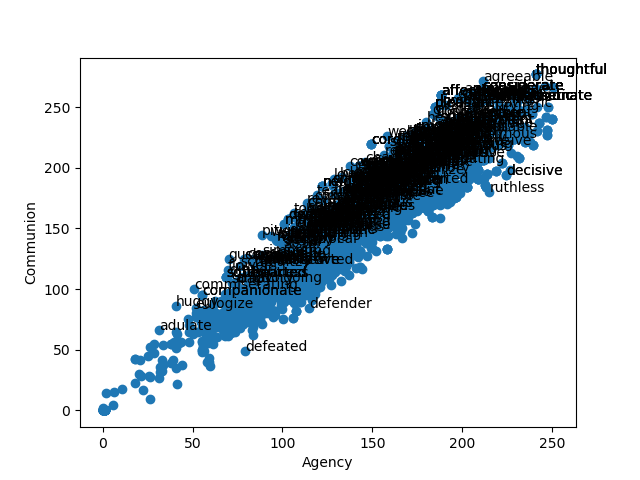
\includegraphics[width=0.8\linewidth]{greater_than30.png}
   \\
    The dots represents all the words in the documents and the words that are labeled were words with an agency vs communion score difference greater than thirty points. The graph labels words based on their word distance similarity to synonyms of the words that fall under the themes of agency vs communion. The graph illustrates words in the document likely to be associate with descriptions of the theme of agency vs communion. \\
    Additionally we examined the quantities of words such as I, love, and you, in authors who had both samples of letter and autobiographies. The diagrams were created by taking counts chapter by chapter in the case of autobiographies or letter by letter in the case of letters. The diagrams illustrate an almost complete lack of the word love in his life document while almost ever letter uses the word love at least once. The maximum usage of the word I was less than a count of sixty five in letter five while the average chapter seems to have at least sixty five instances of the word I. Although this counting metric is very weak in revealing direct motives, attributes of self mastery, and inward versus outward focus. It still is able to illuminate the great difference between a "social" document like a letter and a memoir or autobiography type document.
    \\
    \begin{center}
       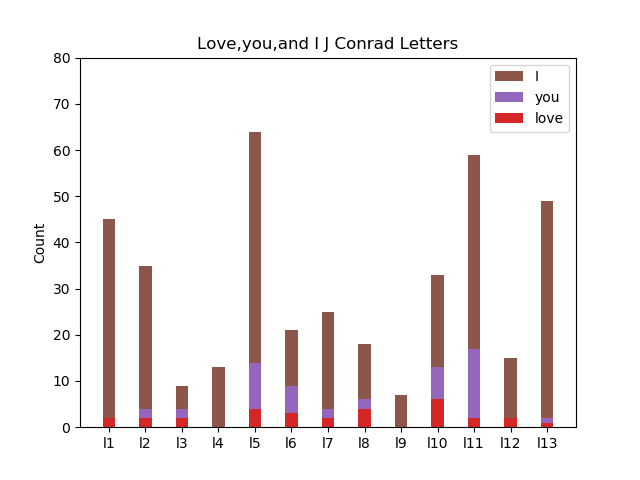
\includegraphics[width=0.8\linewidth]{j_conrad_letters.png}
        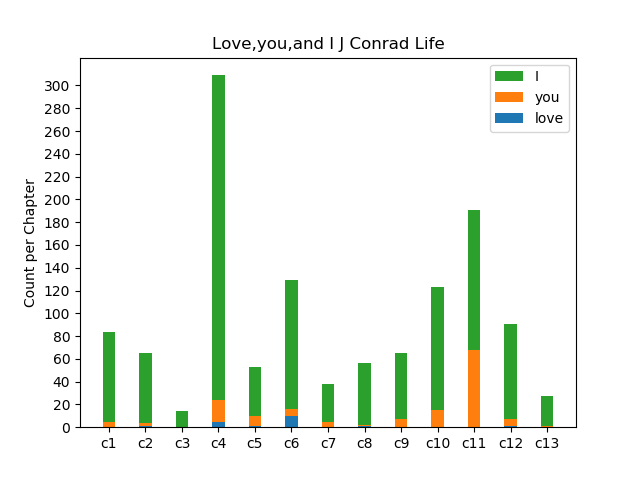
\includegraphics[width=0.8\linewidth]{j_conrad_life.png}
    \end{center}

\section*{Conclusion}
To conclude, our method was able to illuminate words related with the themes of communion and agency in all documents. The words that would be displayed on the edges of the graph or at the max of the scores would be enough to not only illuminate locations in the text but also some of the subject matter in the documents. The words concord, yellow, french, and defeat may seem unrelated to the untrained eye but were all related to the topic of war. 

In addition we looked at some of the ratios of common words used in examples where an author had a biography and letters in order to see how there writing style differed. This helped to illuminate a clear and obvious trends like an increase in the usage of the word I in biographies versus letters. Other trends that would be present are repetition of words colloquially used in letter writing related to the distribution the author chooses, in contrast to the the more diverse less repetitive distribution of words autobiography writers choose to use. 

\section*{Future Work}
Moving forward the first task would be creating a more balanced synonym list using the advisement of subject matter experts. The list of synonyms had more communion words and higher scoring communion words as well. The unbalanced distribution of communion versus agency words lead to issues the unbalanced nature of the main communion versus agency graph.   This can be seen in a zoomed in photo of the graph above in the communion section. Additionally we were uncertain of how to continue when the distribution of words had duplicates meaning some words had co-synonyms. We were uncertain of how to handle this and it is a topic worth examining. Possibly a dimensionality reduction scientist might wish to examine the ability to represent an agency and communion score using the fewest possible word vectors.  \\
\begin{center}
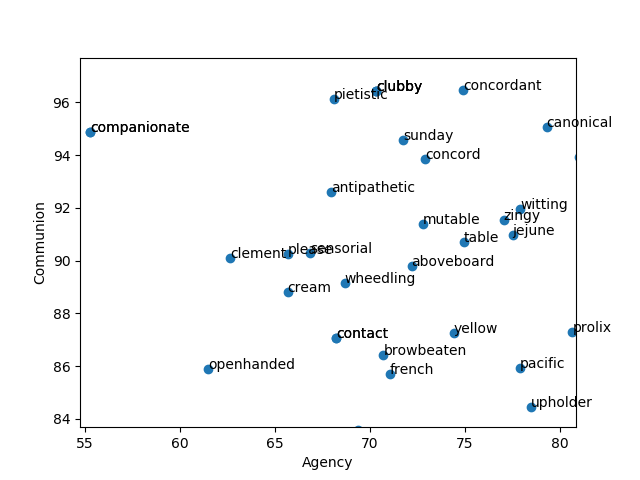
\includegraphics[width=0.8\linewidth]{communion_agency.png}\\
\end{center}
Many odd words ended up being classified as relatively highly communion over agency based in the middle even though they are a little off base. It seems communion drew in some words associated with cowardice. Hopefully by using a more balanced set of synonyms and possibly adding an antonym metric a better more balanced graph could be generated. It would also make sense to explore adapting the synonyms to match those of the period specifically being examined and to look into creating word embeddings using documents more temporally related to the documents being examined. Another task would be searching for words not directly linked with agency or communion but associated with "revelations" of either theme. If the documents were examined for locations of both theme and revelation it would increase the odds of finding true locations in documents where clear examples of the themes of agency versus communion are displayed in the agents in the document. Finally it would go without saying that creating custom word embedding from documents created during the time to go with the custom synonym list for the themes of agency and communion in the time period would be best practice.

\subsection*{Acknowledgments}

We would like to thank Dr. Shannon Quinn and Dr. Elizabeth Davis for assigning this project. We would also like to thank Sydney Panetta, Taylor Morris, Chase Olson, and Oren Morgan who helped give us information and direction on agency and communion. I would also like to thank thesaurus.com for their synonyms and spacy.io for their word embedding which made this project possible.

\section*{References}

\medskip

\small
[1] Bakan, D. (1966): {\it The Duality of Human Existence}. Chicago: Rand McNally and Co. 

[2] Manfred Diehl, Stephanie K. Owen \ \& Lise M. Youngblade \ (2004): {\it Agency and communion attributes in adults’ spontaneous self-representations}, National Institutes of Health.

[3] Andrea E. Abele \ \& Bogdan Wojciszke (2007): {\it Agency and Communion From the Perspective of Self Versus Others}, American Psychological Association.

[4] Bogdan Wojciszke \ \& Olga Bialobrzeska (2014): {\it Agency versus Communion as Predictors of Self-esteem: Searching for the Role of Culture and Self-construal}, Polish Psychological Bulletin.

[5] Vicki S. Helgeson \ \& Heidi L. Fritz (1999): {\it Unmitigated Agency and Unmitigated Communion: Distinctions
from Agency and Communion}, Journal of Research in Personality 33, 131–158.

[6] Dan P. McAdams (2002): {\it Coding Systems for Themes of Agency and Communion}, Northwestern University.

[7] Jochen E. Gebauer, Jenny Wagner,
Constantine Sedikides, \ \& Wiebke Neberich (2013): {\it Agency-Communion and Self-Esteem Relations Are Moderated by Culture, Religiosity, Age, and Sex: Evidence for the “Self-Centrality Breeds Self-Enhancement” Principle}, Journal of Personality, Wiley Periodicals Inc. 

[8] Tomas Mikolov, Kai Chen, Greg Corrado \ \& Jeffrey Dean (2013): {\it Efficient Estimation of Word Representations in Vector Space}, Cornell University.

[9] Tomas Mikolov, Ilya Sutskever, Kai Chen, Gregory Corrado \ \& Jeffrey Dean (2013): {\it Distributed Representations of Words and Phrases and their Compositionality}, Neural Information Processing Systems.

[10] Ben Schmidt (2015): {\it Vector Space Models for the Digital Humanities}, http://bookworm.benschmidt.org/posts/2015-10-25-Word-Embeddings.html.

[11] Vijay Prakash Dwivedi \ \& Manish Shrivastava (2017): {\it Beyond Word2Vec: Embedding Words and Phrases in Same Vector Space}, International Conference on Natural Laguage Processing.

[12] Heuser Ryan (2017):{\it Word Vectors in the Eighteenth Century, Blog },
http://ryanheuser.org

[13] Siobhan Grayson1, Maria Mulvany, Karen Wade, Gerardine Meaney \ \& Derek Greene1 (2016): {\it Novel2Vec: Characterising 19th Century Fiction
via Word Embeddings}, Artificial Intelligence and Cognitive Science.

[14] Arthur Spirling \ \& Pedro L. Rodriguez: {\it Word Embeddings: What works, what doesn’t, and how to tell the difference for applied research}, New York University, Vanderbilt University and Instituto de Estudios Superiores de Administracion.

[15] Agnieszka Pietraszkiewicz, Magdalena Formanowicz, Marie Gustafsson Senden, Ryan L. Boyd, Sverker Sikstrom \ \& Sabine Sczesny (2018): {\it The Big Two Dictionaries: Capturing Agency and Communion in Natural Language}, European Journal of Social Psychology.
\end{document}